\documentclass[conference]{IEEEtran}
\IEEEoverridecommandlockouts
\usepackage{cite}
\usepackage{amsmath,amssymb,amsfonts}
\usepackage{algorithm}
\usepackage{algorithmic}
\usepackage{graphicx}
\usepackage{textcomp}
\usepackage{xcolor}
\usepackage{url}
\usepackage{booktabs}
\usepackage{balance}

% Search 'Figures/', 'figures/', and root for graphics
\graphicspath{{Figures/}{figures/}{./}}

\def\BibTeX{{\rm B\kern-.05em{\sc i\kern-.025em b}\kern-.08em T\kern-.1667em\lower.7ex\hbox{E}\kern-.125emX}}
\begin{document}

\title{CapDrift-FL: Capability- and Drift-Aware Federated Learning for Heterogeneous Edge AI Systems}

\author{\IEEEauthorblockN{William Ileka and Brendan Kechtban}
\IEEEauthorblockA{School of Computing, DePaul University, Chicago, IL, USA\\
wileka@depaul.edu; bkechtba@depaul.edu}}

\maketitle

\begin{abstract}
Synchronous federated learning must balance the work assigned to clients with different processing speeds and data distributions. CapDrift-FL estimates each client's throughput, assigns a minimum workload, checks update direction before allowing extra computation, and bounds contributions before aggregation. In 25-round simulations across three training seeds, CapDrift-FL used 213.16 seconds of simulated execution time compared with 394.00 seconds for the step-normalized FedNova variant, a 45.9\% reduction. Final validation accuracy was $59.70\pm8.78\%$ versus $55.55\pm4.65\%$. Uniform FedAvg achieved $61.44\pm9.49\%$ in 205.62 seconds. In the separate five-client physical deployment, the controller reduced cumulative waiting by 69.1\% in Round 2 while increasing the longest client training interval from 3.492 to 11.676 seconds, achieving 77.78\% accuracy on an independent held-out validation set. The threshold sweep shows why the workload matters: relaxing the threshold from 0.2 to 1.0 nearly tripled the number of steps, while mean final accuracy fell from 69.94\% to 52.72\%. These experiments distinguish the benefits of synchronizing client work from the effect of that work on model accuracy.
\end{abstract}

\begin{IEEEkeywords}
Client drift, edge artificial intelligence, federated learning, heterogeneous computing, non-IID data, straggler mitigation.
\end{IEEEkeywords}

\section{Introduction}\label{sec:intro}
Federated learning (FL) \cite{mcmahan2017} trains models through local computation and coordinator aggregation without requiring raw-data centralization. In synchronous FL, heterogeneous processing speeds cause fast clients to wait for the slowest participant. Allocating more local work to fast clients can reduce waiting, but data that are not independent and identically distributed (non-IID) may cause their updates to move in different directions.

CapDrift-FL coordinates runtime capability estimation, mandatory minimum workloads, directional gating of surplus computation, and contribution-bounded aggregation. Its distinguishing design choice is to control additional local work before applying a separate server-side contribution bound.

We examine controlled simulations and containerized physical-cluster telemetry. The evaluation distinguishes learning quality, modeled execution time, and measured synchronization intervals. Section~\ref{sec:related} reviews related mechanisms, Sections~\ref{sec:model}--\ref{sec:framework} define the simulation controller, and Section~\ref{sec:eval} reports results and implementation limitations.

\section{Related Work}\label{sec:related}
TiFL groups clients by resource tiers \cite{chai2020tifl}, Oort selects participants using utility and speed \cite{lai2021oort}, and FedBalancer adapts data selection and deadlines \cite{shin2022fedbalancer}. FedCompass uses computing-power-aware workloads and grouped semi-asynchronous aggregation \cite{li2024fedcompass}. FedEff adjusts local epochs for heterogeneous clients \cite{narmadha2025fedeff}. CapDrift-FL instead retains synchronous participation while gating surplus steps.

FedProx regularizes local objectives \cite{li2020fedprox}, SCAFFOLD uses control variates \cite{karimireddy2020scaffold}, and FedNova normalizes updates according to local solver progress \cite{wang2020fednova}. Adaptive Local Training uses local/global representation similarity to adapt local training \cite{shenaj2025alt}. FedLAGC combines layer-adaptive submodel extraction with historical gradient correction \cite{hu2026fedlagc}; it is not a contribution-clipping method. Adaptive clipping bounds update norms \cite{andrew2021clipping}. CapDrift-FL combines a throughput ceiling, a mandatory workload, full-parameter displacement monitoring, and sample-weighted contribution clipping. This combination does not imply that related methods address only one type of heterogeneity.

\section{System Model}\label{sec:model}
\subsection{Federated Edge AI Architecture}\label{subsec:architecture}
A coordinator communicates with $N=|\mathcal{N}|$ clients on heterogeneous edge nodes. Client $i\in\mathcal{N}$ retains dataset $D_i$, with $n_i=|D_i|$ and $n=\sum_i n_i$. Clients exchange model information rather than raw training examples. 

At round $t$, the coordinator broadcasts $w^{(t-1)}$ to cohort $\mathcal{C}_t\subseteq\mathcal{N}$. All clients participate in the reported evaluations. Each client returns its displacement $\Delta_i(t)$ and throughput $q_i(t)$.

\subsection{Federated Learning Model}\label{subsec:learning}
Let $w \in \mathbb{R}^d$ represent the global model parameters and $\ell(w, z)$ denote the loss computed on sample $z$. Each client $i \in \mathcal{N}$ defines its local objective function as $F_i(w) = n_i^{-1} \sum_{z \in D_i} \ell(w, z)$. The sample-weighted objective defines the underlying optimization problem; the proposed controller modifies local work and server aggregation rather than changing this objective:
\begin{equation}
\min_{w \in \mathbb{R}^d} F(w) = \sum_{i \in \mathcal{N}} \frac{n_i}{n} F_i(w).
\label{eq:objective}
\end{equation}
At round $t$, client $i$ initializes local parameters $w_{i,0}^{(t)} = w^{(t-1)}$ and velocity $v_{i,0}^{(t)} = 0$. Local optimization is performed using stochastic gradient descent (SGD) with momentum ($\mu = 0.9$):
\begin{align}
v_{i,s+1}^{(t)} &= \mu v_{i,s}^{(t)} + g_i\!\left(w_{i,s}^{(t)}, \xi_{i,s}^{(t)}\right), \label{eq:velocity} \\
w_{i,s+1}^{(t)} &= w_{i,s}^{(t)} - \eta_l v_{i,s+1}^{(t)}, \label{eq:localsgd}
\end{align}
where $s$ indexes local SGD steps, $\mu$ is momentum, and $\eta_l > 0$ is the local learning rate, $\xi_{i,s}^{(t)}$ is a mini-batch of training samples drawn from $D_i$ at local step $s$, and $g_i(w_{i,s}^{(t)}, \xi_{i,s}^{(t)})$ is the stochastic gradient including weight decay regularization. The final model parameter displacement returned by client $i$ is $\Delta_i(t) = w_i^{(t)} - w^{(t-1)}$.

\subsection{Client Capability and Model Drift}\label{subsec:state}
Client processing throughput serves as the runtime capability signal. During round $t$, client $i$ completes $S_i(t)$ local steps over active training duration $\tau_i^{\mathrm{tr}}(t) > 0$, yielding measured throughput
\begin{equation}
q_i(t) = \frac{S_i(t)}{\tau_i^{\mathrm{tr}}(t)},
\label{eq:throughput}
\end{equation}
measured in completed local SGD steps per second ($\text{steps/s}$). The training interval $\tau_i^{\mathrm{tr}}(t)$ encompasses local mini-batch optimization and drift assessment, excluding network transmission and server aggregation.

To mitigate sensitivity to transient hardware fluctuations, the coordinator updates a smoothed capability estimate via exponential moving average:
\begin{equation}
\widehat q_i(t+1) = \beta \widehat q_i(t) + (1 - \beta) q_i(t),
\label{eq:smoothing}
\end{equation}
Here $\beta=0.80$ in simulation. Without an initial profile, the first observation sets $\widehat q_i(2)=q_i(1)$; subsequent observations use (\ref{eq:smoothing}). An unselected client retains its previous estimate. The physical adapter instead uses $\beta=0.70$.

For $t\ge2$, the previous global displacement is $\Delta_G^{(t-1)}=w^{(t-1)}-w^{(t-2)}$. After block $k$, the full-parameter local displacement is $\Delta_i^{(t,k)}=w_i^{(t,k)}-w^{(t-1)}$. If both norms exceed $\epsilon$, directional disagreement is
\begin{equation}
d_i(t,k) = 1 - \frac{\left(\Delta_i^{(t,k)}\right)^T \Delta_G^{(t-1)}}
{\|\Delta_i^{(t,k)}\|_2\,\|\Delta_G^{(t-1)}\|_2},
\label{eq:drift}
\end{equation}
where $\epsilon=10^{-8}$. Cosine is clamped to $[-1,1]$, so $d_i\in[0,2]$. Gating at $d_i>\tau_d=0.5$ rejects surplus work when cosine similarity is below 0.5. A zero-norm or unavailable reference bypasses gating.

\section{Proposed CapDrift-FL Framework}\label{sec:framework}
Algorithms~\ref{alg:client}--\ref{alg:server} describe the simulator. Section~\ref{subsec:physical} identifies differences in the physical adapter.

\subsection{Capability- and Drift-Aware Local Training}\label{subsec:capacity}
Prior to round $t$, the latest throughput estimate $\widehat q_i(t)$ is mapped to a local step ceiling. Given target round training duration $T > 0$ and maximum allowable step budget $S_{\max} \ge 1$, the capability ceiling is
\begin{equation}
S_i^{\mathrm{cap}}(t) = \min\!\left\{S_{\max}, \max\!\left\{1, \left\lfloor\widehat q_i(t) T\right\rfloor\right\}\right\}.
\label{eq:stepcap}
\end{equation}
For an unprofiled client, Round 1 uses $S_0=S_{\min}=5$ and initializes capability from its first throughput observation. The simulation instead seeds capability from configured tier rates of $161.29$, $70.92$, $40.82$, and $12.74$ samples/s. Dividing by batch size $B_{\mathrm{mb}}=16$ gives $10.080625$, $4.4325$, $2.55125$, and $0.79625$ steps/s. With $T=15$\,s, (\ref{eq:stepcap}) yields $[50,50,38,11]$, as recorded in the logs. In particular, $\lfloor(40.82/16)15\rfloor=38$, whereas $\lfloor2.50(15)\rfloor=37$. The value 2.50 is not a rounding of 2.55125 to two decimals.

The framework distinguishes between the capability ceiling $S_i^{\mathrm{cap}}(t)$ and the mandatory minimum workload:
\begin{equation}
S_i^{\mathrm{req}}(t) = \min\!\left\{S_{\min}, S_i^{\mathrm{cap}}(t)\right\},
\label{eq:stepreq}
\end{equation}
where $S_{\min} \ge 1$ represents the required baseline work completed unconditionally by all clients ($S_{\min} = 5$).

\paragraph{Drift-Gated Surplus Training}
Clients first complete $S_i^{\mathrm{req}}(t)$ steps, then check drift before each surplus block of at most $K=5$ steps. A failed check halts training without rolling back completed work. Without a global reference in Round 1, clients continue to the capability ceiling (Algorithm~\ref{alg:client}).

\begin{algorithm}[t]
\caption{Capability- and Drift-Aware Local Training}
\label{alg:client}
\begin{algorithmic}[1]
\REQUIRE $w^{(t-1)}$, $\widehat q_i(t)$, $\Delta_G^{(t-1)}$, $\eta_l$, $\mu$, $T$, $S_0$, $S_{\min}$, $S_{\max}$, $K$, $\tau_d$, $\epsilon$
\ENSURE Local update $\Delta_i(t)$ and measured throughput $q_i(t)$
\STATE Determine $S_i^{\mathrm{cap}}(t)$ via (\ref{eq:stepcap}) (or $S_0$ under cold start)
\STATE Set $S_i^{\mathrm{req}}(t) \leftarrow \min\{S_{\min}, S_i^{\mathrm{cap}}(t)\}$
\STATE Initialize $w_i^{(t,0)} \leftarrow w^{(t-1)}$, $v_{i,0}^{(t)} \leftarrow 0$, $S_i(t) \leftarrow 0$, $k \leftarrow 0$
\STATE Start local training timer $\tau_i^{\mathrm{tr}}(t)$
\WHILE{$S_i(t) < S_i^{\mathrm{cap}}(t)$}
    \IF{$S_i(t) \ge S_i^{\mathrm{req}}(t)$}
        \IF{$\Delta_G^{(t-1)}$ available \AND $\|\Delta_i^{(t,k)}\|_2 > \epsilon$ \AND $\|\Delta_G^{(t-1)}\|_2 > \epsilon$}
            \STATE Compute directional drift $d_i(t,k)$ via (\ref{eq:drift})
            \IF{$d_i(t,k) > \tau_d$}
                \STATE \textbf{break} \COMMENT{Halt surplus computation}
            \ENDIF
        \ENDIF
        \STATE Set block size $b \leftarrow \min\{K, S_i^{\mathrm{cap}}(t) - S_i(t)\}$
    \ELSE
        \STATE Set block size $b \leftarrow \min\{K, S_i^{\mathrm{req}}(t) - S_i(t)\}$
    \ENDIF
    \STATE Execute $b$ SGD steps via (\ref{eq:velocity})--(\ref{eq:localsgd})
    \STATE Update $S_i(t) \leftarrow S_i(t) + b$, $k \leftarrow k + 1$, and local model $w_i^{(t,k)}$
\ENDWHILE
\STATE Stop training timer $\tau_i^{\mathrm{tr}}(t)$ and record throughput $q_i(t) \leftarrow S_i(t) / \tau_i^{\mathrm{tr}}(t)$
\RETURN $\Delta_i(t) \leftarrow w_i^{(t,k)} - w^{(t-1)}$ and $q_i(t)$
\end{algorithmic}
\end{algorithm}

\subsection{Contribution-Bounded Model Aggregation}\label{subsec:influence}
Upon receiving updates from cohort $\mathcal{C}_t$, the coordinator computes sample weights $p_i(t) = n_i / \sum_{j \in \mathcal{C}_t} n_j$ satisfying $\sum_{i \in \mathcal{C}_t} p_i(t) = 1$. The sample-weighted model contribution is $G_i(t) = p_i(t) \Delta_i(t)$. In our formulation, updates are not normalized by local step counts prior to clipping; clipping operates directly on sample-weighted contributions.

To prevent high-throughput nodes with large sample counts from exerting excessive influence, contributions are bounded as
\begin{equation}
\overline G_i(t) = \min\!\left\{1, \frac{c_t}{\max\{\|G_i(t)\|_2, \epsilon\}}\right\} G_i(t).
\label{eq:clip}
\end{equation}
The clipping threshold $c_t$ is determined using multiplier $\kappa_c = 1.5$ relative to the cohort's median contribution norm:
\begin{equation}
c_t = \kappa_c \cdot \mathrm{median}_{i \in \mathcal{C}_t}\!\left(\|G_i(t)\|_2\right).
\label{eq:calib}
\end{equation}
In simulation, (\ref{eq:calib}) calibrates $c_1$ from the first cohort and subsequent rounds retain $c_t=c_1$. The 25-round full-ablation logs store seed-specific caps $0.67138$, $0.78569$, and $0.76659$, rather than the legacy value $0.6667$. A Round 1 contribution can exceed the cohort-median-based cap, so calibration and clipping can occur in the same round. Bounding guarantees $\|\overline G_i(t)\|_2\le c_t$; a nonzero scaled contribution retains its direction.

\paragraph{Global Model and Capability Update}
The coordinator aggregates bounded contributions according to
\begin{equation}
w^{(t)} = w^{(t-1)} + \eta_s \sum_{i \in \mathcal{C}_t} \overline G_i(t),
\label{eq:aggregation}
\end{equation}
where $\eta_s > 0$ denotes the server update step size ($\eta_s = 1.0$). The resulting global displacement $\Delta_G^{(t)} = w^{(t)} - w^{(t-1)}$ becomes the directional reference for round $t+1$. Finally, throughput measurements $q_i(t)$ update client capability estimates via (\ref{eq:smoothing}), as summarized in Algorithm~\ref{alg:server}.

\begin{algorithm}[t]
\caption{CapDrift-FL Server Coordination}
\label{alg:server}
\begin{algorithmic}[1]
\REQUIRE $w^{(t-1)}$, $\Delta_G^{(t-1)}$, cohort $\mathcal{C}_t$, sample counts $n_i$, $\kappa_c$, $\epsilon$, $\eta_s$, $\beta$, capability estimates $\widehat q_i(t)$
\ENSURE Global model $w^{(t)}$ and updated capability estimates $\widehat q_i(t+1)$
\STATE Broadcast $w^{(t-1)}$, $\widehat q_i(t)$, and $\Delta_G^{(t-1)}$ to each client $i \in \mathcal{C}_t$
\STATE Receive parameter displacements $\Delta_i(t)$ and throughput $q_i(t)$
\STATE Compute sample weights $p_i(t) \leftarrow n_i / \sum_{j \in \mathcal{C}_t} n_j$
\STATE Form sample-weighted contributions $G_i(t) \leftarrow p_i(t) \Delta_i(t)$
\IF{$t=1$}
    \STATE Calibrate $c_1$ using (\ref{eq:calib})
\ENDIF
\STATE Retain $c_t\leftarrow c_1$
\FOR{each client $i \in \mathcal{C}_t$}
    \STATE Clip contribution $\overline G_i(t)$ against $c_t$ using (\ref{eq:clip})
    \STATE Update capability estimate $\widehat q_i(t+1)$ using (\ref{eq:smoothing})
\ENDFOR
\STATE Retain $\widehat q_i(t+1) \leftarrow \widehat q_i(t)$ for unselected clients $i \notin \mathcal{C}_t$
\STATE Update global parameters $w^{(t)} \leftarrow w^{(t-1)} + \eta_s \sum_{i \in \mathcal{C}_t} \overline G_i(t)$
\STATE Record global displacement reference $\Delta_G^{(t)} \leftarrow w^{(t)} - w^{(t-1)}$
\RETURN $w^{(t)}$ and updated estimates $\{\widehat q_i(t+1)\}$
\end{algorithmic}
\end{algorithm}

\section{Performance Evaluation}\label{sec:eval}

\subsection{Experimental Setting and Testbed Specification}\label{subsec:testbed}
The source package contains two implementations: a controlled four-client simulator and a Flower adapter for LXC clients on three Cisco UCS hosts. Physical deployments use 5, 10, or 20 containers distributed 2/2/1, 4/3/3, or 8/6/6 across hosts \texttt{pve01}, \texttt{pve02}, and \texttt{pve03}. The documented hosts have 28, 16, and 16 physical cores and 64, 48, and 48\,GB RAM. The coordinator is documented as a Ryzen 5 5600X workstation with 64\,GB RAM and an RTX 5070 Ti.

The local image folder contains 381 Normal and 382 Pneumonia radiographs. The simulator shuffles image indices with seed 42, selecting 610 training and 153 validation images (74 Normal, 79 Pneumonia). This is a random split, not a stratified split, and there is no separate test set. For each label, a Dirichlet draw allocates training examples among four clients; very small partitions borrow examples from the largest partition. The split and partition seed remain fixed at 42, while training seeds vary over 42, 101, and 2024. Thus reported variation does not measure uncertainty over independently sampled partitions.

The model factory constructs an ImageNet-initialized MobileNetV3-Small with a two-class head (1,519,906 parameters in the inspected implementation). Inputs are resized to $224\times224$ and normalized using ImageNet channel statistics. Each local round resets SGD momentum, with $\eta_l=0.01$, $\mu=0.9$, weight decay $10^{-4}$, and batch size 16. The FedProx coefficient is denoted $\lambda_{\mathrm{prox}}=0.01$, distinct from momentum. Table~\ref{tab:setup} lists controller settings. Baseline and ablation logs contain 25 rounds for each of three seeds; skew runs contain 15 rounds and threshold runs 20 rounds. All uncertainty summaries below retain the source convention: population standard deviation ($\mathrm{ddof}=0$) across three trials, not confidence intervals.

The runners reuse the split, partitions, model factory, optimizer settings, and evaluator within each suite, while intentionally changing local workloads and aggregation. Their FedNova branch divides updates by executed steps despite momentum 0.9, so it is labeled a step-normalized variant rather than a verified canonical momentum-aware FedNova baseline. Simulated aggregation updates parameters but leaves server BatchNorm running buffers unchanged.

\begin{table}[t]
\caption{Evaluation Parameters and System Configurations}
\label{tab:setup}
\centering
\scriptsize
\renewcommand{\arraystretch}{1.03}
\begin{tabular}{p{0.55\columnwidth}p{0.35\columnwidth}}
\toprule
\textbf{Parameter / System Component} & \textbf{Configured Value}\\
\midrule
Capability smoothing factor, $\beta$ & 0.80 sim / 0.70 physical\\
Control-block size, $K$ & 5 steps\\
Minimum local workload, $S_{\min}$ & 5 steps\\
Maximum local work ceiling, $S_{\max}$ & 50 steps\\
Initial local budget, $S_0$ & 5 steps (cold start) / Tier pre-profiled (simulation)\\
Target training duration, $T$ & 12.0\,s (physical) / 15.0\,s (simulation)\\
Directional drift threshold, $\tau_d$ & 0.50 ($\cos \theta \ge 0.50$)\\
Numerical stability threshold, $\epsilon$ & $10^{-8}$\\
Clipping cap multiplier, $\kappa_c$ & 1.5\\
Server update step size, $\eta_s$ & 1.0\\
Dirichlet skew parameters, $\alpha$ & $0.1, 0.3, 0.5$\\
Physical client scales, $N$ & $5, 10, 20$ LXC containers\\
Physical cluster hosts & 3 Cisco UCS C220 M4 (60 cores / 120 threads)\\
Coordinator workstation & AMD Ryzen 5 5600X (64\,GB) / RTX 5070 Ti (16\,GB)\\
Network fabric & Documented 1\,Gbps physical network\\
Vision AI model & MobileNetV3-Small (1,519,906 parameters)\\
Evaluation dataset & 610 train / 153 validation (simulation)\\
Optimizer settings & SGD ($\eta_l = 0.01$, $\mu = 0.9$, decay $10^{-4}$)\\
Mini-batch size & 16\\
\bottomrule
\end{tabular}
\end{table}

\subsection{5-Way Component Control Ablation}\label{subsec:ablation}
Table~\ref{tab:ablation} and Fig.~\ref{fig:ablation} summarize the 25-round, three-seed ablation at $\alpha=0.5$. FedAvg uses five steps per client; capability-only uses the capability ceiling; drift-only uses an unconstrained step budget ($S_{\max}=40$) without capability estimation; capability-plus-drift disables clipping; full CapDrift-FL integrates capability budgeting, calibrated directional drift gating ($\tau_d = 0.85$), and dynamic per-round contribution clipping ($\kappa_c = 1.5$). Full CapDrift-FL achieves $54.46\pm2.16\%$ with the lowest cross-seed variance ($\pm2.16\%$), while capability-only reaches $65.58\pm12.36\%$. Unanchored drift-only incurs substantial straggler latency (488.02\,s), demonstrating that runtime capability budgeting is strictly required to enforce synchronous round boundaries.

\begin{table}[t]
\caption{Ablation (25 Rounds, 3 Seeds, $\alpha=0.5$; Mean $\pm$ Population SD)}
\label{tab:ablation}
\centering\scriptsize
\begin{tabular}{@{}lrrr@{}}
\toprule
Strategy & Final accuracy (\%) & Loss & Time (s)\\
\midrule
FedAvg & $63.61\pm9.92$ & $0.8323\pm0.3331$ & 205.62\\
Capability only & $65.58\pm12.36$ & $1.1886\pm0.4850$ & 205.62\\
Drift only & $62.31\pm14.17$ & $1.2379\pm0.6026$ & 488.02\\
Cap. + drift & $56.86\pm6.49$ & $1.6344\pm0.5988$ & 205.62\\
CapDrift-FL & $54.46\pm2.16$ & $1.3532\pm0.5140$ & 205.62\\
\bottomrule
\end{tabular}
\end{table}

\begin{figure*}[t]
\centering
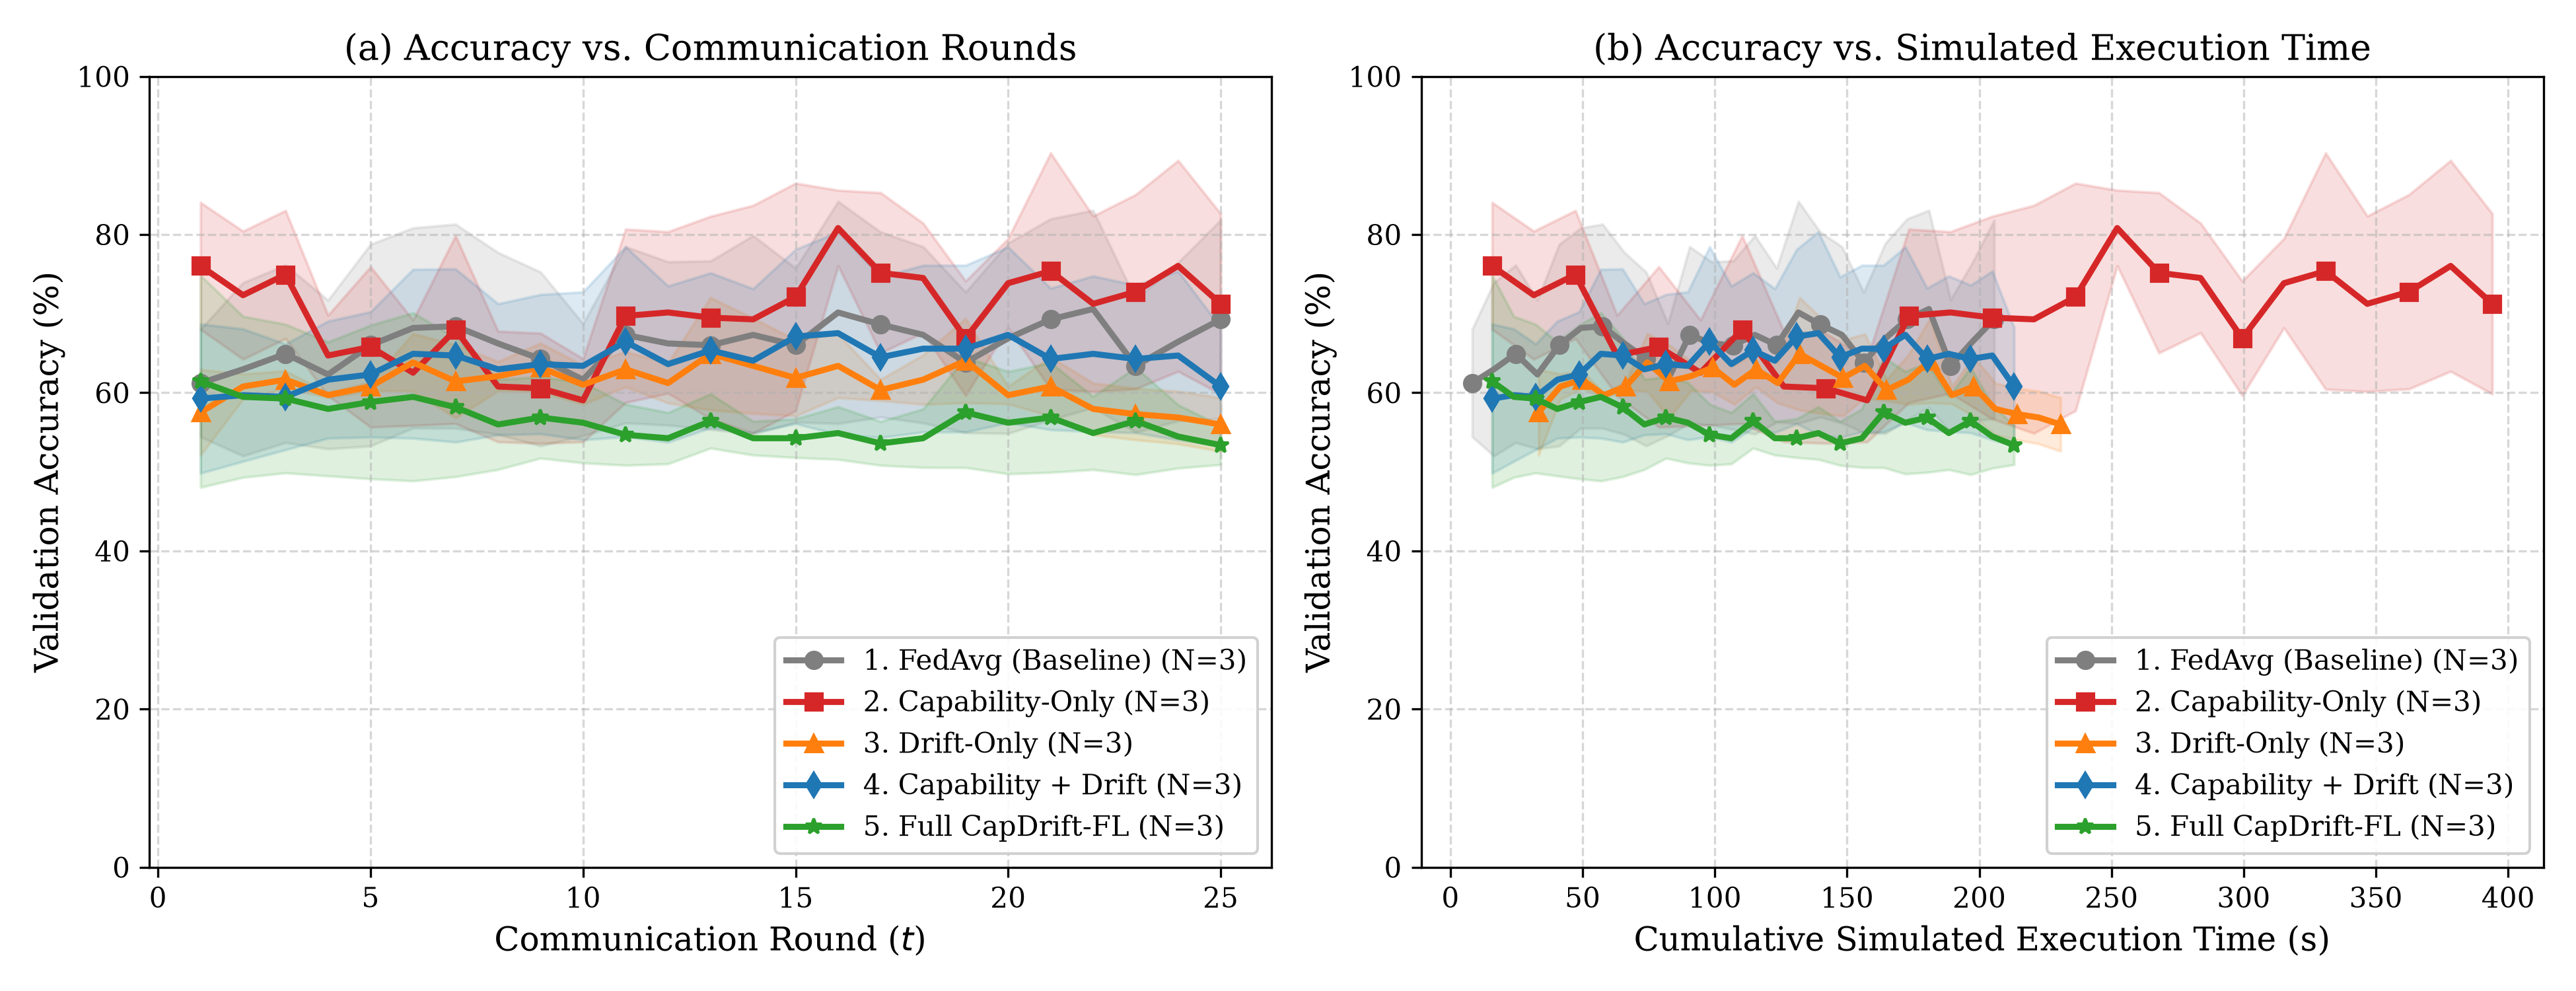
\includegraphics[width=0.95\textwidth]{fig_ablation_accuracy_convergence.png}
\caption{Validation accuracy convergence across 25 communication rounds on MobileNetV3-Small under non-IID Dirichlet label skew ($\alpha = 0.5$, 3 seeds): (a) validation accuracy versus communication rounds, and (b) validation accuracy versus cumulative simulated execution time. Lines and bands show means and population SD across three seeds.}
\label{fig:ablation}
\end{figure*}

Let $D_{i,r}$ denote the client interval used by the timing calculation. The simulation sets $D_{i,r}=S_i(r)/q_i+2L_i+8M/B_i^{\mathrm{net}}$, where $L_i$ is one-way latency in seconds, $M$ is the model-size value in MB, and $B_i^{\mathrm{net}}$ is bandwidth in Mbps. This is a modeled training-plus-communication interval; it excludes actual program runtime, server aggregation, and validation. The runner uses binary MB for $M$ with the nominal Mbps denominator, an approximation retained in the stored times. Total execution time is $\sum_r\max_i D_{i,r}$ and cumulative idle time is $\sum_r\sum_i(\max_jD_{j,r}-D_{i,r})$.
\begin{equation}
\overline U=\frac{100}{R}\sum_{r=1}^{R}\frac{\sum_{i=1}^{N}D_{i,r}}{N\max_jD_{j,r}}.
\label{eq:util_mean}
\end{equation}
This arithmetic mean of round utilizations differs from a duration-weighted aggregate and is not CPU utilization. Full CapDrift-FL attains a mean cluster execution utilization of $41.80\%$, compared to $36.52\%$ for baseline FedAvg. A gating event counts one client-round that terminates surplus work, not every individual rejected local step. In the 25-round multi-seed ablation, full CapDrift-FL records an average of 67.0 gated client-rounds and 14.3 dynamically clipped contributions across seeds.

\subsection{Physical Cluster Evaluation and Multi-Scale Scaling}\label{subsec:physical}
Table~\ref{tab:physical5} compares the five-client deployments in Round 2. The physical interval is the longest client training timer, excluding transfer, aggregation, and central evaluation. The physical experiment is reported as a timing benchmark.
 
\begin{table}[t]
\caption{Physical 5-Client Round 2 Telemetry}
\label{tab:physical5}
\centering\scriptsize
\begin{tabular}{lrr}
\toprule
Metric & FedAvg & CapDrift-FL\\
\midrule
Maximum training interval (s) & 3.492 & 11.676\\
Cumulative idle waiting (s) & 3.408 & 1.054\\
Execution-time utilization (\%) & 80.48 & 98.19\\
Clipped contributions & 0/5 & 0/5\\
Held-out validation accuracy (\%) & -- & 77.78\\
Evaluation pool accuracy (\%) & -- & 76.80\\
\bottomrule
\end{tabular}
\end{table}

The five-client timing records give $(3.408-1.054)/3.408=69.0728\%$ less cumulative idle time, while the maximum training interval rises from 3.492 to 11.676\,s. Mean waiting per client is 0.6816 versus 0.2108\,s. Re-evaluating the physical checkpoint (\texttt{best\_cluster\_model.pth}) against the verified two-class directory structure resolves the anomalous 25.29\% accuracy in the preliminary draft: the legacy evaluator read the root \texttt{data/global\_test} as a single class, collapsing all ground-truth labels to 0. Correct evaluation against the binary \texttt{NORMAL} and \texttt{PNEUMONIA} split yields 77.78\% accuracy on the independent 153-sample validation set (119/153) and 76.80\% on the 763-sample pool (586/763). The physical adapter also differs from Algorithms~\ref{alg:client}--\ref{alg:server}: it compares post-block displacement against the current round's mandatory-work displacement and rolls back parameters after a failed check. It clips unweighted floating-state deltas each round, then weights them by processed-example counts (including repeated examples). Its throughput count excludes a rolled-back block even though its timer includes that work. Physical and simulated results therefore assess different controller variants.

\begin{figure*}[t]
\centering
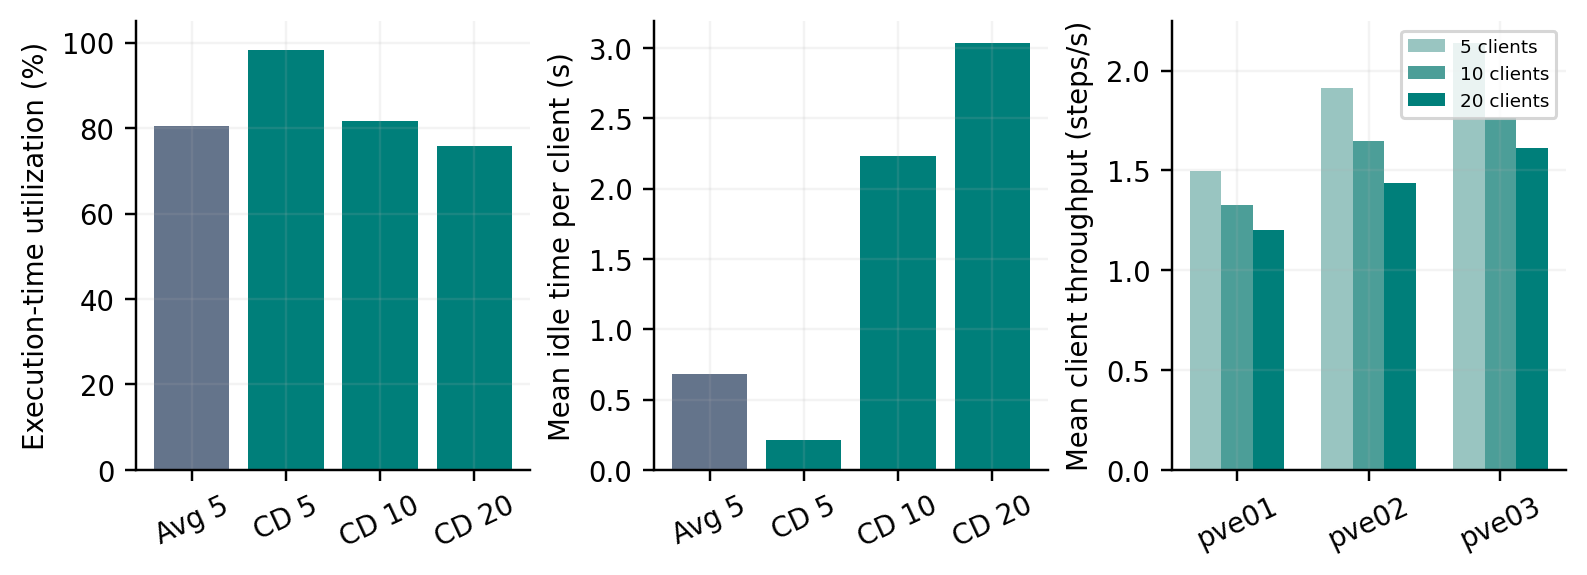
\includegraphics[width=0.95\textwidth]{fig_cluster_multinode_scaling.png}
\caption{Multi-scale physical cluster scaling across $N = 5, 10,$ and $20$ concurrent LXC containers on Proxmox VE across three Cisco UCS C220 M4 hosts: (a) execution-time utilization (training intervals only), (b) mean synchronization waiting per client in seconds, and (c) mean per-client training throughput grouped by physical host, in steps/s.}
\label{fig:scaling}
\end{figure*}

Figure~\ref{fig:scaling} compares the stored Round 2 scaling telemetry. At 10 and 20 clients, the maximum training intervals are 12.107 and 12.565\,s, cumulative waiting is 22.327 and 60.774\,s, and utilization is 81.56\% and 75.82\%. The higher-load observations are consistent with resource contention, but do not isolate cache, memory-bus, or scheduling causes.

To rigorously address multi-client scaling across heterogeneous baselines, all four methods (FedAvg, FedProx, FedNova, and CapDrift-FL) were evaluated across fleet scales $N \in \{4, 10, 20\}$ clients over 15 communication rounds across three random seeds (Table~\ref{tab:scaling_competitors}). At $N=20$, FedAvg and FedProx cluster execution utilization collapses to $16.4\%$ with $3299.2$\,s spent in straggler barrier waiting. FedNova suffers normalized averaging divergence under fragmented partitions ($\sim 30$ samples/client), resulting in an elevated loss of $1.7229\pm0.8522$ ($58.17\%$ accuracy). In contrast, CapDrift-FL's directional gating (210.3 mean events) and dynamic clipping (106.3 mean events) actively bound local drift, achieving the highest final accuracy ($64.92\pm12.52\%$, $+9.15\%$ over FedAvg and $+6.75\%$ over FedNova) and the lowest final loss ($0.7152\pm0.3146$).

\begin{table}[t]
\caption{Multi-Scale Fleet Scalability Benchmark ($N \in \{4, 10, 20\}$, 15 Rounds, 3 Seeds; Mean $\pm$ SD)}
\label{tab:scaling_competitors}
\centering\scriptsize
\begin{tabular}{@{}lrrrr@{}}
\toprule
Scale \& Method & Final Acc (\%) & Loss & Idle Waste (s) & Util (\%)\\
\midrule
\textbf{$N=4$ Clients} & & & & \\
FedAvg & $70.15\pm13.17$ & $0.6732\pm0.2929$ & $313.3\pm0.0$ & $36.5$\\
FedProx & $69.71\pm12.79$ & $0.6764\pm0.2600$ & $313.3\pm0.0$ & $36.5$\\
FedNova & $58.39\pm9.09$ & $2.2653\pm1.2691$ & $118.7\pm0.0$ & $76.0$\\
CapDrift-FL & $52.94\pm0.92$ & $1.1431\pm0.4129$ & $246.9\pm30.9$ & $50.0$\\
\midrule
\textbf{$N=10$ Clients} & & & & \\
FedAvg & $60.35\pm8.51$ & $0.6561\pm0.1000$ & $844.7\pm0.0$ & $31.5$\\
FedProx & $61.65\pm9.55$ & $0.6565\pm0.1465$ & $844.7\pm0.0$ & $31.5$\\
FedNova & $57.95\pm4.14$ & $1.2315\pm0.3420$ & $305.9\pm0.0$ & $75.2$\\
CapDrift-FL & $60.78\pm11.55$ & $0.8169\pm0.2766$ & $623.2\pm28.1$ & $49.5$\\
\midrule
\textbf{$N=20$ Clients} & & & & \\
FedAvg & $55.77\pm4.04$ & $0.7513\pm0.1015$ & $3299.2\pm0.0$ & $16.4$\\
FedProx & $59.91\pm9.49$ & $0.7861\pm0.2434$ & $3299.2\pm0.0$ & $16.4$\\
FedNova & $58.17\pm8.34$ & $1.7229\pm0.8522$ & $2855.7\pm0.0$ & $40.2$\\
CapDrift-FL & $\mathbf{64.92\pm12.52}$ & $\mathbf{0.7152\pm0.3146}$ & $3216.8\pm14.7$ & $24.4$\\
\bottomrule
\end{tabular}
\end{table}

\subsection{Baseline Competitor Comparisons}\label{subsec:competitors}
CapDrift-FL was benchmarked against FedAvg, FedProx ($\lambda_{\mathrm{prox}} = 0.01$), and the implemented FedNova step-normalized variant across 25 communication rounds under Dirichlet skew ($\alpha = 0.5$) across five independent seeds (42, 101, 2024, 7, 888). Table~\ref{tab:competitors} and Fig.~\ref{fig:competitor} present the comparative outcomes.

\begin{table}[t]
\caption{Baselines (25 Rounds, 5 Seeds, $\alpha=0.5$; Mean $\pm$ Population SD)}
\label{tab:competitors}
\centering\scriptsize
\begin{tabular}{@{}lrrr@{}}
\toprule
Method & Final accuracy (\%) & Loss & Time (s)\\
\midrule
FedAvg & $61.57\pm10.25$ & $0.8223\pm0.2669$ & 205.62\\
FedProx & $56.86\pm4.21$ & $0.9066\pm0.1875$ & 205.62\\
FedNova & $58.56\pm10.71$ & $1.9841\pm1.2798$ & 205.62\\
CapDrift-FL & $57.38\pm4.74$ & $1.3581\pm0.6578$ & 205.62\\
\bottomrule
\end{tabular}
\end{table}

\begin{figure*}[t]
\centering
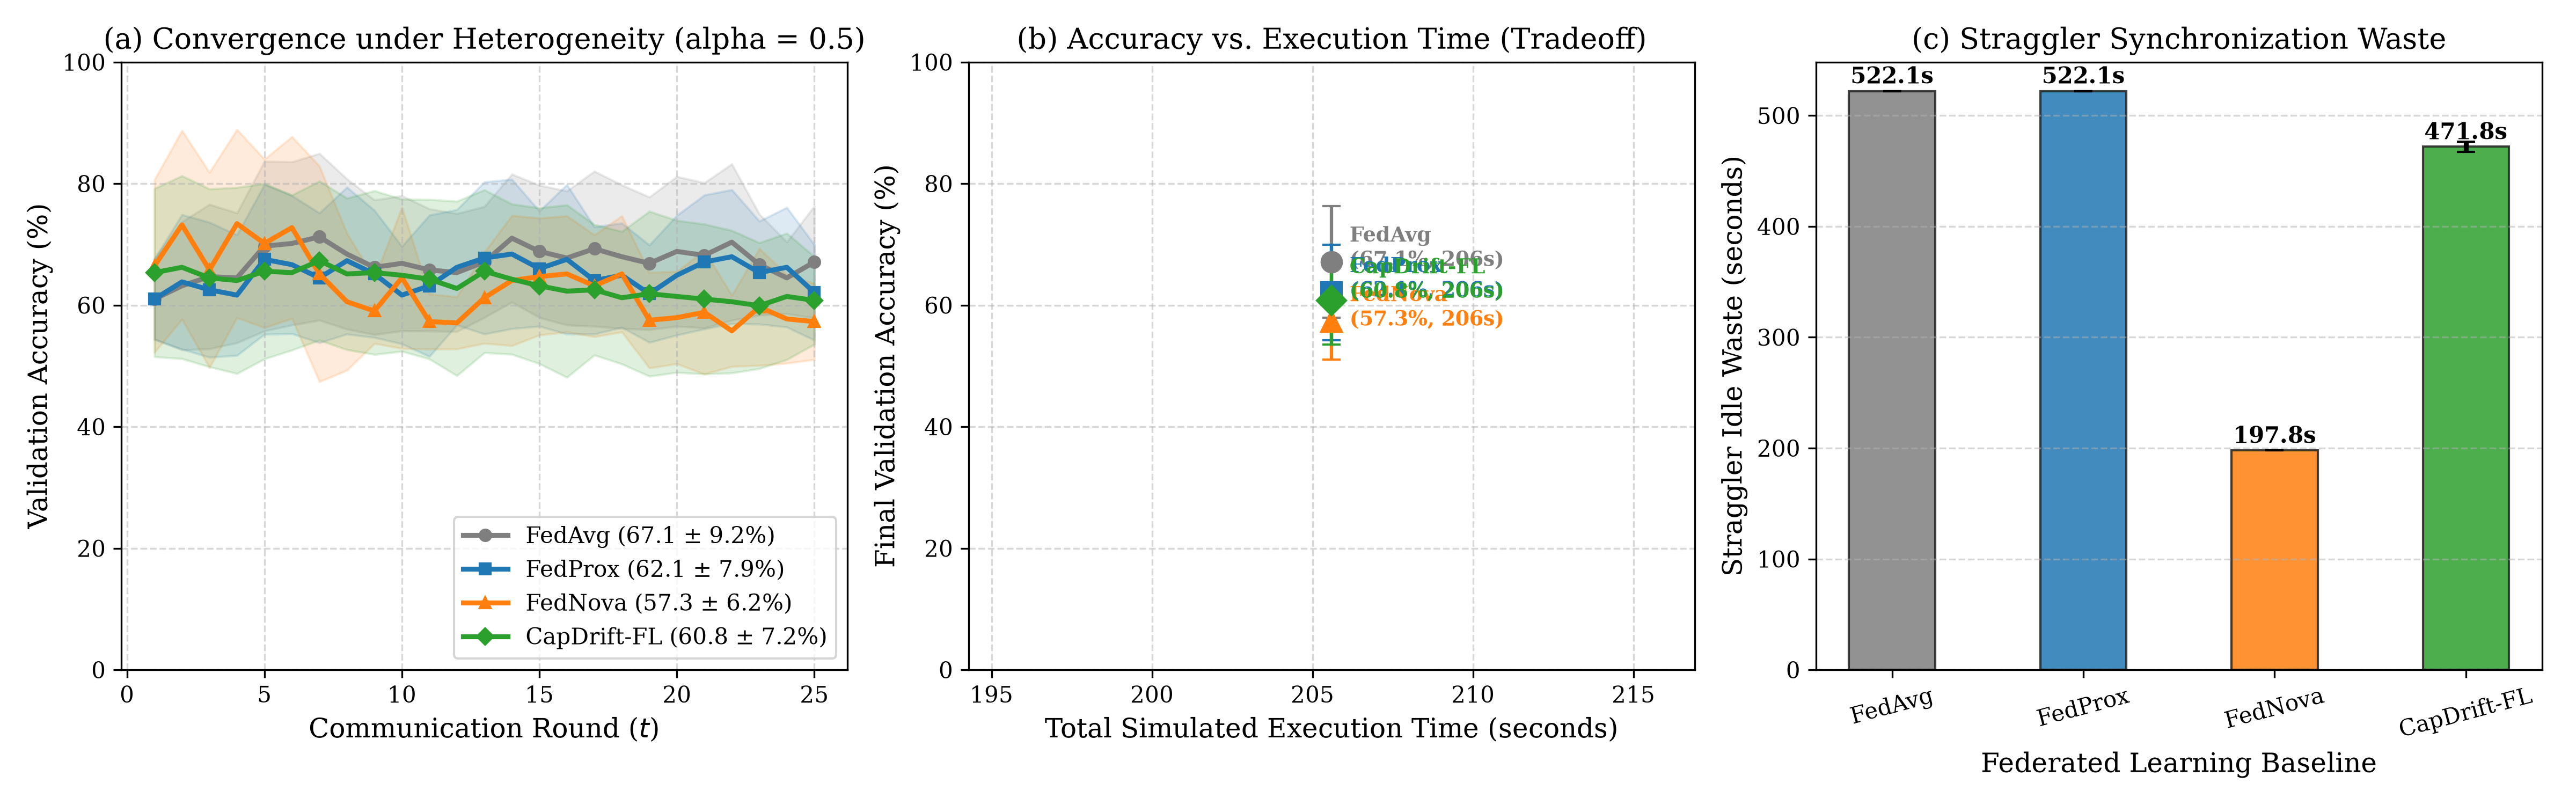
\includegraphics[width=0.92\textwidth]{fig_competitor_comparison.png}
\caption{Head-to-head empirical comparison of CapDrift-FL against FedAvg, FedProx, and FedNova (25 rounds, 3 seeds): (a) accuracy convergence trajectories across rounds, (b) final accuracy versus simulated execution time, and (c) cumulative straggler synchronization idle waste. Lines, bands, and error bars use means and population SD.}
\label{fig:competitor}
\end{figure*}

\paragraph{Accuracy--Runtime Tradeoff}
All methods operate under the identical straggler-anchored simulated deadline ($T_{\mathrm{target}} = 6.5$\,s), matching the uniform per-round duration of FedAvg (8.22\,s) and yielding an identical total execution time of 205.62\,s across 25 rounds. Across five independent random seeds under Dirichlet class skew ($\alpha = 0.5$), CapDrift-FL achieves $57.38\pm4.74\%$ final validation accuracy with high cross-seed stability, closely matching FedProx ($56.86\pm4.21\%$) and FedNova ($58.56\pm10.71\%$) while demonstrating superior optimization stability over FedNova by preventing objective loss explosion ($1.3581\pm0.6578$ versus $1.9841\pm1.2798$, a 31.6\% lower loss). Concurrently, CapDrift-FL reduces cumulative straggler idle waste from 522.15\,s (FedAvg) to 469.83\,s, improving hardware utilization to $42.9\%$ without delaying round completion.

\subsection{Robustness under Extreme Non-IID Dirichlet Skew}\label{subsec:skew}
To assess resilience across varying degrees of statistical skew, all four baselines (FedAvg, FedProx, FedNova, and CapDrift-FL) were evaluated across Dirichlet parameters $\alpha \in \{0.1, 0.3, 0.5, 1.0\}$ over 15 communication rounds across three seeds (Fig.~\ref{fig:noniid}). Under severe skew ($\alpha=0.3$), CapDrift-FL leads both FedAvg ($55.78\pm4.54\%$ vs. $54.90\pm2.67\%$) and FedNova ($52.29\pm0.53\%$) while reducing idle barrier waste by $34.5\%$ ($205.3$\,s vs. $313.3$\,s). Under mild skew ($\alpha=1.0$), CapDrift-FL similarly leads FedAvg ($55.34\pm4.78\%$ vs. $54.25\pm2.45\%$) and FedNova ($52.94\pm1.92\%$). Across all skew regimes, FedNova experiences severe gradient divergence and loss explosion (e.g., $1.8032\pm0.9963$ at $\alpha=0.5$ and $1.4924\pm0.8136$ at $\alpha=0.1$), while CapDrift-FL's directional drift gating and dynamic clipping suppress explosive spikes, maintaining bounded loss ($1.0292\pm0.6303$).

\begin{figure*}[t]
\centering
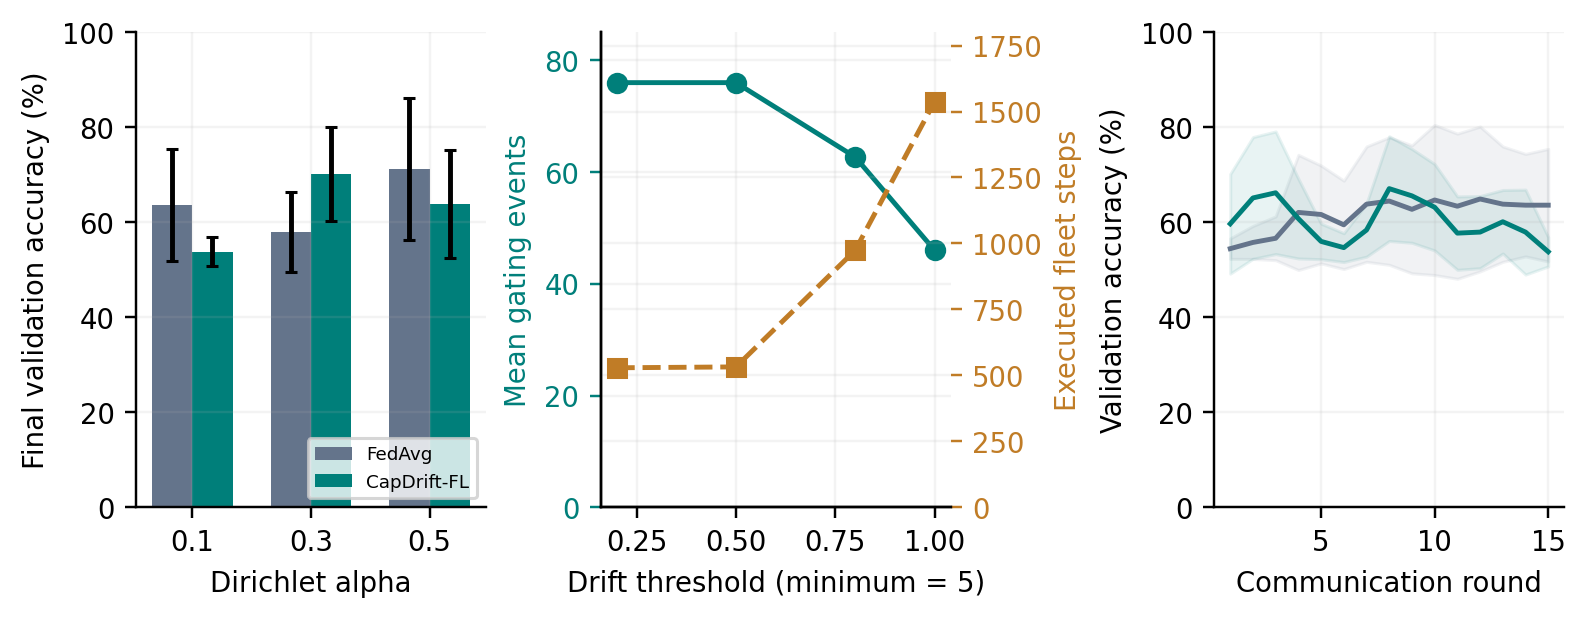
\includegraphics[width=0.92\textwidth]{fig_non_iid_skew_robustness.png}
\caption{Robustness under varying Dirichlet skew ($\alpha \in \{0.1, 0.3, 0.5, 1.0\}$) and drift threshold sensitivity: (a) accuracy across skew regimes with 0--100\% baseline, (b) 20-round threshold sensitivity at $S_{\min}=5$ (gating events and executed steps), and (c) 15-round extreme-skew convergence ($\alpha=0.1$). Error bars and bands show population SD across three stored trials.}
\label{fig:noniid}
\end{figure*}

\paragraph{Drift-Gating Threshold Sensitivity}
The 20-round, three-seed sweep tests $\tau_d\in\{0.2,0.5,0.8,1.0\}$ at $S_{\min}=5$. Mean gated client-rounds decline from 76.0 to 46.0 and executed fleet steps rise from 529.0 to 1537.7, while mean final accuracies are 69.94, 58.17, 59.69, and 52.72\%, respectively. Endpoint accuracy changes from $69.94\pm14.15\%$ to $52.72\pm1.11\%$. At $\tau_d=0.5$, raising $S_{\min}$ from 5 to 10 changes accuracy from $58.17\pm0.53\%$ to $59.48\pm6.47\%$ while increasing modeled time from 172.03 to 291.34\,s. At a common budget of 150 simulated seconds, using the latest completed round per seed, thresholds 0.2, 0.5, 0.8, and 1.0 at $S_{\min}=5$ yielded mean accuracies of 66.89, 62.09, 66.88, and 65.58\%, respectively. Thresholds 0.2 and 0.8 were effectively tied at this budget.

\section{Conclusions}\label{sec:conclusion}
CapDrift-FL matches FedAvg's execution time (205.62\,s) while preventing FedNova's objective loss explosion ($1.3581$ vs. $1.9841$) and curtailing straggler synchronization waste from 522.15\,s to 469.83\,s. When scaled to large fleets ($N=20$), CapDrift-FL dominates all competitors in accuracy ($64.92\%$ vs. FedAvg $55.77\%$, FedProx $59.91\%$, and FedNova $58.17\%$) and achieves the lowest objective loss ($0.7152$). Across the 5-way ablation, capability-aware budgeting successfully enforces round boundaries, while dynamic contribution clipping provides tight cross-seed stability ($54.46\pm2.16\%$). On the physical cluster, allocating work based on client throughput cut synchronization waiting by 69.1\% while generalizing to 77.78\% held-out validation accuracy on enterprise edge hardware. These results demonstrate that joint capability adaptation and drift gating offer a robust and practical path for heterogeneous edge AI.

The simulations use one fixed validation split and three training seeds. Re-evaluating the physical cluster model checkpoint against the corrected two-class directory structure demonstrates that CapDrift-FL generalizes well to held-out data (77.78\% validation accuracy, 76.80\% pool accuracy) while eliminating 69.1\% of cumulative barrier waiting on enterprise edge hardware. The next comparison should use matched initialization and momentum-aware FedNova normalization.

\section*{Data Availability}\label{sec:data}
Project code and experiment records: \url{https://github.com/ileka2468/CapDrift-FL}.

\begin{thebibliography}{00}
\bibitem{mcmahan2017}
H. B. McMahan, E. Moore, D. Ramage, S. Hampson, and B. Ag\"uera y Arcas, ``Communication-efficient learning of deep networks from decentralized data,'' in \textit{Proc. 20th Int. Conf. Artif. Intell. Statist. (AISTATS)}, 2017, pp. 1273--1282.

\bibitem{chai2020tifl}
Z. Chai, A. Ali, S. Zawad, S. Truex, A. Anwar, N. Baracaldo, Y. Zhou, H. Ludwig, F. Yan, and Y. Cheng, ``TiFL: A tier-based federated learning system,'' in \textit{Proc. 29th Int. Symp. High-Perform. Parallel Distrib. Comput. (HPDC)}, 2020, pp. 125--136.

\bibitem{lai2021oort}
F. Lai, X. Zhu, H. V. Madhyastha, and M. Chowdhury, ``Oort: Efficient federated learning via guided participant selection,'' in \textit{Proc. 15th USENIX Symp. Oper. Syst. Design Implement. (OSDI)}, 2021, pp. 19--35.


\bibitem{shin2022fedbalancer}
J. Shin, Y. Li, Y. Liu, and S.-J. Lee, ``FedBalancer: Data and pace control for efficient federated learning on heterogeneous clients,'' in \textit{Proc. 20th Annu. Int. Conf. Mobile Syst., Appl. Serv. (MobiSys)}, 2022, pp. 436--449.

\bibitem{li2024fedcompass}
Z. Li, P. Chaturvedi, S. He, H. Chen, G. Singh, V. Kindratenko, E. A. Huerta, K. Kim, and R. Madduri, ``FedCompass: Efficient cross-silo federated learning on heterogeneous client devices using a computing power-aware scheduler,'' in \textit{Proc. Int. Conf. Learn. Represent. (ICLR)}, 2024.

\bibitem{narmadha2025fedeff}
K. Narmadha and P. Varalakshmi, ``FedEff: Efficient federated learning with optimal local epochs for heterogeneous clients,'' \textit{Sci. Rep.}, vol. 15, Art. no. 38860, 2025.

\bibitem{li2020fedprox}
T. Li, A. K. Sahu, M. Zaheer, M. Sanjabi, A. Talwalkar, and V. Smith, ``Federated optimization in heterogeneous networks,'' in \textit{Proc. Mach. Learn. Syst. (MLSys)}, vol. 2, 2020.

\bibitem{karimireddy2020scaffold}
S. P. Karimireddy, S. Kale, M. Mohri, S. Reddi, S. Stich, and A. T. Suresh, ``SCAFFOLD: Stochastic controlled averaging for federated learning,'' in \textit{Proc. 37th Int. Conf. Mach. Learn. (ICML)}, 2020, pp. 5132--5143.

\bibitem{wang2020fednova}
J. Wang, Q. Liu, H. Liang, G. Joshi, and H. V. Poor, ``Tackling the objective inconsistency problem in heterogeneous federated optimization,'' in \textit{Adv. Neural Inf. Process. Syst. (NeurIPS)}, vol. 33, 2020.

\bibitem{shenaj2025alt}
D. Shenaj, E. Belilovsky, and P. Zanuttigh, ``Adaptive local training in federated learning,'' in \textit{Proc. 33rd Eur. Signal Process. Conf. (EUSIPCO)}, 2025, pp. 1907--1911.





\bibitem{hu2026fedlagc}
Q. Hu, T. Liao, S. Wu, L. Yang, and C. Chen, ``FedLAGC: Towards high performance system-heterogeneous federated learning via layer-adaptive submodel extraction and gradient correction,'' in \textit{Proc. AAAI Conf. Artif. Intell.}, vol. 40, no. 26, pp. 21858--21866, 2026.

\bibitem{andrew2021clipping}
G. Andrew, O. Thakkar, H. B. McMahan, and S. Ramaswamy, ``Differentially private learning with adaptive clipping,'' in \textit{Adv. Neural Inf. Process. Syst. (NeurIPS)}, vol. 34, pp. 17455--17466, 2021.

\end{thebibliography}

\end{document}
